% \Huge

\todo[inline]{Introduce cosmic variance somewhere}

\section{Perturbation Theory}

\subsection{Overview}

The evolution of primordial perturbations into the structure we detect today is studied analytically using Perturbation Theory (PT). This field can be divided, according to the frame used to study the Universe, into Eulerian PT and Lagrangian PT (LPT). In the Eulerian frame the evolution of the spatial distribution of particles is studied (\cite{Bernardeau_PT}). On the other hand, in the Lagrangian frame, particles are tracked and their evolution with time is studied.

The Eulerian frame has been so widely used to study the growth of perturbations, that we refer to it as Standard Perturbation Theory (e.g. \cite{1983MNRAS.203..345V}, \cite{peebles1980large}). The most popular approach is to consider an irrotational fluid characterized by its overdensity and peculiar velocity distributions (\cite{Carlson_perturbation_theory}). However, this method suffers from divergences at large wavenumbers (on small scales). This lead to a number of extensions meant to bring it under control (\cite{2006PhRvD..73f3519C},~\cite{2008PhRvD..77b3533C}). 

Lagrangian Perturbation Theory has been well developed in the 1990s (\cite{1992MNRAS.254..729B},~\cite{1993MNRAS.264..375B},~\cite{1994MNRAS.267..811B}). However, it has received less attention partly because the method breaks down after shell-crossing (\cite{Carlson_perturbation_theory}). This event will be discussed further in Section 2.2. Recently it has been demonstrated that LPT correctly reproduces the SPT power spectrum, but also even it's linear first order approximation correctly predicts the decay of the correlation between the final (non-linear) and the initial fields (\cite{2008PhRvD..77f3530M},~\cite{2008PhRvD..78h3519M}). As this correlation is the main tool used in this project, our main focus is on the Lagrangian Frame. 

\subsection{The Zel'dovich Approximation}

The central object of Lagrangian Perturbation Theory is the displacement field $\Psi(\textbf{q})$ which maps the initial particle positions expressed by the Lagrangian coordinate $\textbf{q}$ to the final Eulerian particle positions $\textbf{x}$ (\cite{Bernardeau_PT}):
\begin{equation}
     \textbf{x}(t) = \textbf{q} + \Psi(\textbf{q}, t)
\end{equation}

The first order approximation to this equation leads to a separation of variables $\textbf{q}$ and $t$ (\cite{1993sfu..book.....P}). After also adding the expanding background we obtain:
\begin{equation}
    \textbf{r}(t) = a(t) \textbf{x}(t) = a(t) [\textbf{q} + b(t) \textbf{p}(\textbf{q})]
    \label{eq:2.2}
\end{equation}
Where $\textbf{x}(t)$ is now the comoving Eulerian coordinate.

This approximation was first proposed by \cite{1970A&A.....5...84Z} and it now carries his name, as the Zel'dovich Approximation (ZA). It only works for scales much smaller than the horizon, where Newtonian analysis is possible. However, as our purpose is to study the growth of structure on scales smaller than the BAO, this approximation is a very good starting point. 

An important detail is that the ZA (up to a point) works even in the non-linear regime. This regime is defined in terms of the overdensity $\delta$. When $\delta \sim 1$ we enter the non-linear regime. Standard Perturbation Theory generally breaks down at this point. However, by switching to a description in terms of the particle trajectories, we can reach non-linear density contrasts without the particles being perturbed too much (\cite{1993sfu..book.....P}).

On a final note, the ZA is very good at predicting the loss of correlation between the initial and the final density fields (e.g.~\cite{2016PhRvD..93j3519P}). With all these considerations in mind, in this project we will investigate reconstruction methods within the Zel'dovich Approximation.

\section{The non-linear regime}

\subsection{Cosmological simulations}
 However, once we get into the deeply non-linear regime, these methods break down. Instead we rely on large N-body simulations to continue our study of the evolution of structure.

Generally, these simulations are used to help constrain Cosmological theories of the primordial universe or to test perturbation theories. A random initial field with properties based on the CMB and our general understanding of the early universe, is evolved through time until the present. The output of the simulation is then compared to observational data. Simulations like Millennium XXL (\cite{Millennium_XXL}) or Illustris (\cite{Illustris_sim}) gave us an unprecedented insight into structure formation and evolution.

On the other hand, simulations are also used as a laboratory for testing reconstruction methods they give us access to both the initial and the final density fields. We can attempt a reconstruction on the final field and then compare it to the initial field and test how well it worked. 

\subsection{Information loss}


\todo[inline]{Talk about the Linear regime of collapse versus the non-linear regime. Present the difficulty of constructing analytical models of non-linear collapse. Motivate our use of simulations as well as our desire to get back to the linear regime for reconstruction.}

\section{Reconstruction}

This can be understood by thinking about the difference between looking at the large scales versus the small scales. For example, a very large (by scale) primordial underdensity will probably still be an underdensity at late times (as a huge void). However, on small scales, information tends to be destroyed. A small scale primordial underdensity might be caught in the larger bulk flows and collapse in a larger halo. In this case, the information about the small underdensity is lost. \todo{this paragraph could go in chapter 2}


\todo[inline]{Finally link everything with an overview of Reconstruction techniques and how our work fits into the modern context.}

\todo[inline]{Showcase the BAO reconstruction.}

% \begin{figure}
%     \centering
%     %\hspace*{\fill}
%     \subfloat[]{
%       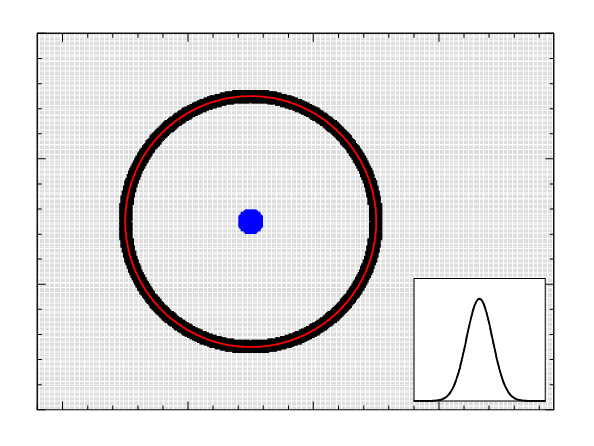
\includegraphics[width=0.45\columnwidth]{images/misc/slice000.png}%
%     }\hfill
%     \subfloat[]{
%       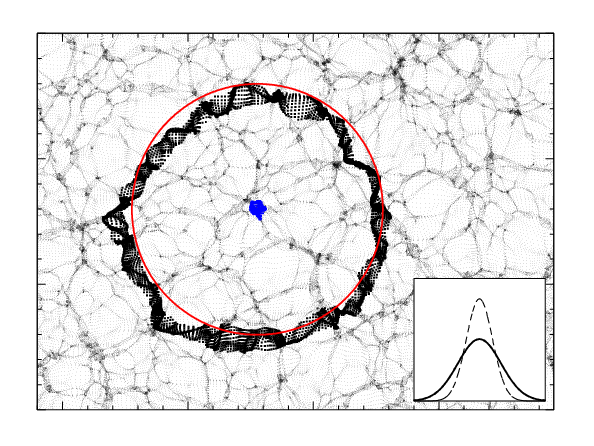
\includegraphics[width=0.45\columnwidth]{images/misc/slice040.png}%
%     }\hfill
%     \subfloat[]{
%       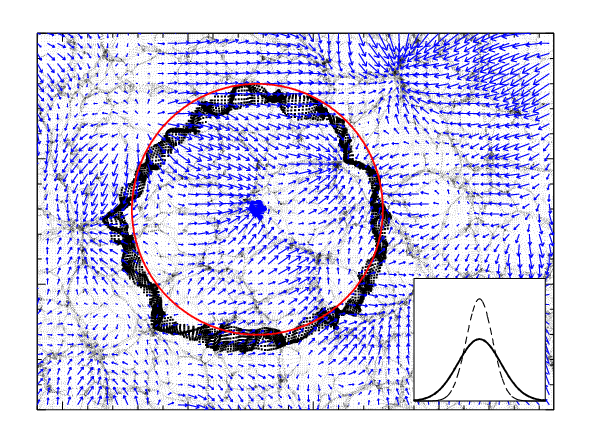
\includegraphics[width=0.45\columnwidth]{images/misc/vector040.png}%
%     }\hfill
%     \subfloat[]{
%       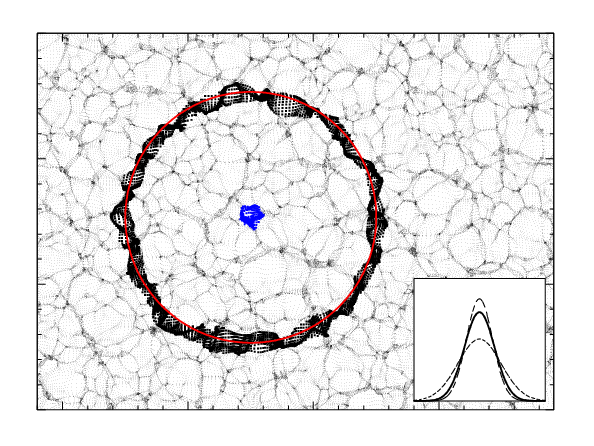
\includegraphics[width=0.45\columnwidth]{images/misc/recon040.png}%
%     }\hfill
    
%     \caption{
%       \setstretch{1.0}
%       \small
%     An illustration taken from~\cite{2012MNRAS.427.2132P}, showing how the acoustic scale is distorted by non-linear effects and then reconstructed. (a) In the early Universe, the density field was very smooth. The acoustic feature is marked with a ring of radius $150Mpc$, and the distance between the centroid (blue point) and the radially distributed black points is represented by a Gaussian. (b) In the late Universe, non-linear effects move the points on the acoustic scale from their original positions (still represented by the red circle). This can be seen as a broadening of the radial distribution (dashed line is the original). The evolution here was modelled using the Zel'dovich approximation. (c) The Lagrangian displacement field (blue arrows) is calculated. The concept behind reconstruction techniques is to estimate the displacement field in order to move the particles back to their original position. The field was smoothed using a Gaussian filter. (d) The particles were moved back along the displacement field, and a clear improvement can be seen. The solid line marks the reconstructed radial distribution, the dashed line represents the primordial distribution, and the dotted line is the late time distribution before reconstruction. In this case the reconstruction is not perfect because of the Gaussian filter, which was used to mimic a real scenario. Note that this was done just for illustration purposes, and actual reconstruction methods are more complex.
%     }
    
% \label{fig:3}
% \end{figure}

% \section{The Matter Power Spectrum}

% As our objective is to reconstruct the final density field and compare it to the initial one, we need a good way of describing the two fields. A widely used method is to look at the Matter Power Spectrum. We first start with the overdensity $\delta$:
% \begin{equation}
%     \delta(\textbf{x}) = \frac{\rho(\textbf{x}) - \overline{\rho}}{\overline{\rho}}
% \end{equation}
% where $\rho(\textbf{x})$ is the density at $\textbf{x}$, and $\overline{\rho}$ is the average density. The spatial average of this overdensity field is not a good characterization as it is equal to 0. Instead we look at its variance, the correlation function:
% \begin{equation}
%     \xi
% \end{equation}